%%%%%%%%%%%%%%%%%%%%%%%%%%%%%%%%%%%%%%%%%%%%%%%%%%%%%%%%%%%%%%%%%%%%%%%%%%%%%%%%%%
\begin{frame}[fragile]\frametitle{}
\begin{center}
{\Large Overview}
\end{center}
\end{frame}

%%%%%%%%%%%%%%%%%%%%%%%%%%%%%%%%%%%%%%%%%%%%%%%%%%%%%%%%%%%%%%%%%%%%%%%%%%%%%%%%%%%
\begin{frame} \frametitle{Why Python?}
\begin{itemize}
\item  Readability.
\item Ease of use.
\item Fits in your head.
\item Gets things done.
\item Good libraries.
\item Lookie what I did!.
\end{itemize}
\end{frame}


%%%%%%%%%%%%%%%%%%%%%%%%%%%%%%%%%%%%%%%%%%%%%%%%%%%%%%%%%%%%%%%%%%%%%%%%%%%%%%%%%%%
\begin{frame}[fragile]  \frametitle{Introduction}
\begin{itemize}
\item Python is a simple, yet powerful interpreted language.
\item  Numerous libraries: NumPy, SciPy, Matplotlib \ldots.
\item Named after Monty Python.
\item Open Source and Free
\item Invented by Guido van Rossum.
\end{itemize}
\end{frame}

%%%%%%%%%%%%%%%%%%%%%%%%%%%%%%%%%%%%%%%%%%%%%%%%%%%%%%%%%%%%%%%%%%%%%%%%%%%%%%%%%%%
\begin{frame}[fragile]\frametitle{Python's Benevolent Dictator For Life}

\adjustbox{valign=t}{
\begin{minipage}{0.5\linewidth}
{\em ``Python is an experiment in how  much freedom programmers need.  Too much freedom and nobody can read another's code; too little and expressiveness is endangered.''}

      - Guido van Rossum 
\end{minipage}
}
\hfill
\adjustbox{valign=t}{
\begin{minipage}{0.4\linewidth}
\begin{center}
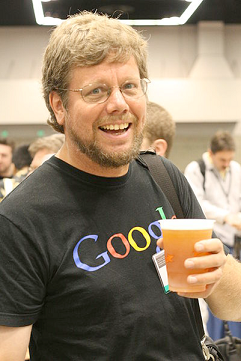
\includegraphics[width=0.8\linewidth,keepaspectratio]{rossum}
\end{center}
\tiny{(Reference: https://en.wikipedia.org/ wiki/Guido\_van\_Rossum)}
\end{minipage}
}
\end{frame}



%%%%%%%%%%%%%%%%%%%%%%%%%%%%%%%%%%%%%%%%%%%%%%%%%%%%%%%%%%%%%%%%%%%%%%%%%%%%%%%%%%%
\begin{frame}[fragile]  \frametitle{What is Python?}
\begin{itemize}
\item Interpreted
\item Object-oriented 
\item High-level
\item Dynamic semantics
\item Cross-platform
\item Readability.
\end{itemize}


\end{frame}


%%%%%%%%%%%%%%%%%%%%%%%%%%%%%%%%%%%%%%%%%%%%%%%%%%%%%%%%%%%%%%%%%%%%%%%%%%%%%%%%%%%
\begin{frame}[fragile]  \frametitle{Compiled Languages}
\begin{itemize}
\item Needs entire program
\item Translates directly to machine codes 
\item Exe native and fast
\item Usually statically typed
\item Types known during compilation
\item Change in type : recompilation
\item Ideal for compute-heavy tasks
\item E.g. C, C++, FORTRAN
\end{itemize}
\end{frame}

%%%%%%%%%%%%%%%%%%%%%%%%%%%%%%%%%%%%%%%%%%%%%%%%%%%%%%%%%%%%%%%%%%%%%%%%%%%%%%%%%%%
\begin{frame}[fragile]  \frametitle{Interpreted Languages}
\begin{itemize}
\item  Interpreted on the fly
\item No need to compile: can execute right away
\item Usually dynamically typed
\item Non-syntax errors are detected only in run-time
\item Slower than compiled languages
\item Ideal for small tasks
\item  E.g. Python, Perl, PHP, Bash
\end{itemize}

Note: Python, at the beginning, loosely checks the program. Only at run time, line-by-line, it checks for errors. So, if the error statements are not in the running path, their error does not get reported. So, its a bit relaxed. Thats the objection for its use in production code, where strong type checking and error checking, upfront is essential.
\end{frame}

%%%%%%%%%%%%%%%%%%%%%%%%%%%%%%%%%%%%%%%%%%%%%%%%%%%%%%%%%%%%%%%%%%%%%%%%%%%%%%%%%%%
\begin{frame}[fragile]  \frametitle{JIT-Compiled Languages}
\begin{itemize}
\item Between compiled and interpreted
\item Code is initially interpreted, hotspots compiled
\item Deduce types during compilation, can change in run-time
\item Slower than compiled
\item E.g. Java, C\#
\end{itemize}
\end{frame}

%%%%%%%%%%%%%%%%%%%%%%%%%%%%%%%%%%%%%%%%%%%%%%%%%%%%%%%%%%%%%%%%%%%%%%%%%%%%%%%%%%%
\begin{frame}[fragile]  \frametitle{``C'' guys to take pride in}
\begin{itemize}
\item Python interpreter written in  ``C''
\item Source code at www.python.org
\item So, Python Interpreter is compiled exe
%\item On windows, its \lstinline|C:\Python35\python.exe|
\end{itemize}
\end{frame}


%%%%%%%%%%%%%%%%%%%%%%%%%%%%%%%%%%%%%%%%%%%%%%%%%%%%%%%%%%%%%%%%%%%%%%%%%%%%%%%%%%%
\begin{frame}[fragile]  \frametitle{Completely Controversial Observations about Languages}
\begin{center}
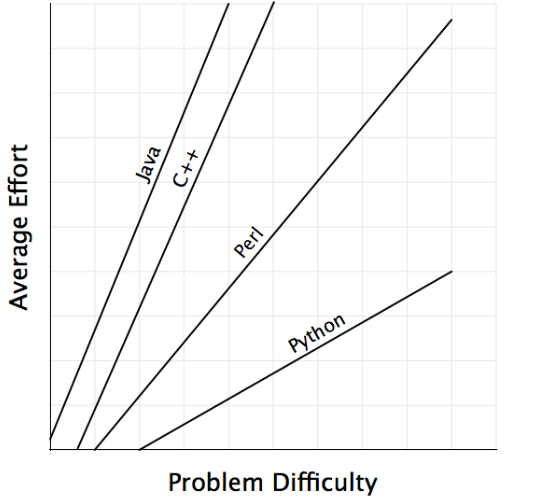
\includegraphics[width=0.6\linewidth,keepaspectratio]{langs}
\end{center}
\end{frame}


%%%%%%%%%%%%%%%%%%%%%%%%%%%%%%%%%%%%%%%%%%%%%%%%%%%%%%%%%%%%%%%%%%%%%%%%%%%%%%%%%%%
\begin{frame}[fragile]  \frametitle{Python Help}
\begin{itemize}
\item Home page -- http://www.python.org
\item Wiki -- http://wiki.python.org/
\item  Packages -- https://pypi.python.org/pypi
\item Projects at http://sourceforge.net and github.org
%\item Import a module, then view its  \lstinline{.__doc__}  attribute.
%\item At the interactive prompt, use  \lstinline{help(obj)}
\end{itemize}
\end{frame}


%%%%%%%%%%%%%%%%%%%%%%%%%%%%%%%%%%%%%%%%%%%%%%%%%%%%%%%%%%%%%%%%%%%%%%%%%%%%%%%%%%%
\begin{frame}[fragile]  \frametitle{Important features}
\begin{itemize}
\item Built-in high level data types: \lstinline{strings, lists, dictionaries}, etc.
\item Usual control structures: \lstinline{if, if-else, if-elif-else, while, for}
\item Levels of organization: \lstinline{functions, classes, modules, packages}
\item Extensions in C and C++ possible
\end{itemize}
\end{frame}

%%%%%%%%%%%%%%%%%%%%%%%%%%%%%%%%%%%%%%%%%%%%%%%%%%%%%%%%%%%%%%%%%%%%%%%%%%%%%%%%%%%
\begin{frame}[fragile]  \frametitle{Python 2 \emph{vs} Python 3}
\begin{itemize}
\item Two major versions 2.*, 3.*
\item Python 2.7: Latest release in 2.x series
\item Python 3.5: More polished syntax, removed inconsistencies
\end{itemize}
\end{frame}
